% \newcommand{\prototitle}{Versuch 2 - Statistik}
% \newcommand{\Fachbereich}{Praktikum Messtechnik}
% \input{../packages/tu_header}

\newcommand{\institut}{Institut f\"ur Telekommunikationssysteme}
\newcommand{\fachgebiet}{Nachrichten\"ubertragung}
\newcommand{\veranstaltung}{Praktikum Nachrichten\"ubertragung}
\newcommand{\pdfautor}{\"Ozg\"u Dogan (326 048), Boris Henckell (325 779)}
\newcommand{\autor}{\"Ozg\"u Dogan (326 048)\\ Boris Henckell (325 779)}
\newcommand{\gruppe}{Gruppe: }
%\newcommand{\betreuer}{Betreuer: Mahmoud Felk}


\newcommand{\pdftitle}{Nachrichten\"ubertragung\ Praktikum\ 01}
\newcommand{\prototitle}{Praktikum 01 \\ Einf\"uhrung in MATLAB}


\input{../../packages/tu_header_8}

%---------------------------------------------------------------------
%---------------------------------------------------------------------
%---------------------------------------------------------------------
\section{Einleitung}

Dieses Praktikum diente hauptsächlich dem Einarbeiten in die Laborumgebung und
dem Umgang der verwendeten Messger\"ate. Außerdem wurde der Einsatz von MatLab
geübt und einige wichtige Signale implementiert und untersucht.


\section{Vorbereitungsaufgaben}

    \begin{quote}
   	
        \subsection{Das Specktrum eines unendlich ausgedehnten Rechteckkamms}
        \begin{quote}
            Das besagt Rechteckkamm setzt sich wie folgt zusammen:
          
            \vspace{1em}
            
            \begin{equation*}
            	\begin{split}
            		u(t) = A \cdot &\sqcap_{\alpha T}(t) \ast \delta_T(t)\ , \\
                    0 < &\alpha < 1
            	\end{split}
            \end{equation*}
          	
          	Die Faltung im Zeitbereich, welche durch den Stern dargestellt wird,
          	entspricht einer Multiplikation der fouriertransformierten Faktoren
          	im Frequenzbereich. Daher gilt:
          	
          	\vspace{1em}
          	
          	\begin{equation*}
            	\begin{split}
            		F\{ A \cdot \sqcap_{\alpha T}(t) \} &= A \alpha T \cdot si(\frac{\omega \alpha T}{2})\\
                    F\{ \delta_T(t) \} &= \omega_T \delta_{\omega_T} (\omega)\\
                    &= \frac{2 \pi}{T} \delta_{\omega_T} (\omega)
            	\end{split}
            \end{equation*}
          	          
          	Daraus folgt:
          	
          	\vspace{1em}
          	
          	\begin{equation*}
            	\begin{split}
            		\Rightarrow
            		F\{ A \cdot &\sqcap_{\alpha T}(t) \ast \delta_T(t)\} = A \alpha T \cdot si(\frac{\omega \alpha T}{2})
            		\cdot \omega_T \delta_{\omega_T} (\omega)
            	\end{split}
            \end{equation*}
          	
   		 \end{quote}  	
	\end{quote}
         	
%--------------------------------------------------------------------
%--------------------------------------------------------------------            
\section{Praktische Aufgaben}

    \begin{quote}
        \subsection{Übungen für den Umgang mit MatLab}
		\begin{quote}
    		\subsubsection{Rechteck}
            \begin{quote}
                Um schnellstmöglich den Umgang mit MatLab zu erlernen, wurde uns eine Datei
                names rechteck.m und Aufgabe1.m vorgegeben. Damit konnten wir einen
                Rechtecksignal der Spannung mit einer Amplitude von 2V und einer
                vorgegebenen Länge simulieren.\\
                Dieses Signal wird anschließend Fourier transformiert. Dannach werden das Signal im Zeitbereich sowie der
                Amplitudengang und der Phasengang des Fourier transformierten Signals geplottet 
                
                \vspace{1em}
                
                Als nächstes wurde der Frequenzbereich für die
                Spektren im Code von Aufgabe1.m so verändert, dass wir den Bereich zwischen $0$
                und $4kHz$ darstellen konnten. Dazu wurden die Achsenwerte für die x-Achse
                (Frequenzbereich) und für die y-Achse (Amplituden) in den plot Befehlen
                überarbeitet.\\
                Außerdem haben wir untersucht, welche Auswirkunden die Veränderung des
                Tastgrads $\alpha$ hat. Die Spektren und Amplituden wurden für die Werte der
                folgenden Tabelle simuliert und untersucht.
                
                \vspace{1em}
                
                    \begin{center}
                         \begin{tabular}{|c|c|c|c|}
                             
                          \hline
                           $\alpha $ & $f[Hz]$ & Amplitude $[V]$ & Signaldauer
                           $T_{ges}[s]$\\ \hline
                           0.1 & 50 & 2 & 0.5 \\ \hline
                           0.5 & 50 & 2 & 0.5 \\ \hline
                           0.9 & 50 & 2 & 0.5 \\ \hline           
           
                         \end{tabular}
                     \end{center}
                  \vspace{1em}
                
                Als nächstes wurde die Amplitude so umgestellt, dass sie in dB angegeben
                wurde. Dies realisierten wir mit der ``log'' Funktion in MatLab, die die
                Umrechnung des Betragsspektrums ermöglicht.\\
                Die Funktion lautete dementsprechend:\\
                
                \begin{equation*}
                    \begin{split}
                        y_{DFT}_{abs} = 10*LOG10(abs(y_DFT)/N);     
                    \end{split}
                \end{equation*}
        
                Mit der ``ylim'' Funktion konnten wir dann die y-Achse zwischen $-30 dB$
                und $5 dB$ limitieren. Dafür verwendeten wir das Kommando:\\
                
                \begin{center}
                
                \begin{align*}
                    ylim ([-30 \ 5]);
                \end{align*}
                
                \end{center}
                
                Der komplette Code rechteck.m und Aufgabe1.m ist im Anhang zu finden.\\
                
            \end{quote}
            
            \subsubsection{Dreieck}
            \begin{quote}
                Nachdem das Rechecksignal abgeschlossen wurde, schreiben wir diesen Code zu
                einer dreieck.m Datei um. Das Ziel dabei war es die Funktion so zu
                modifizieren, dass eine bipolare Dreickfolge erstellt wurde. Der Taskgrad
                $\alpha$ sollte wieder variabel mit den Werten $\alpha = 0.1$, $\alpha = 0.5$
                und $\alpha = 0.9$ sein. Dies gelang uns, indem wir die if-Bedingungen in der
                rechteck.m Datei wie folgt umschrieben:
    
\begin{lstlisting}
if(t_{rel} < alpha*T_{periode})
res(k) = -A+((2*A)*t_{rel}/(alpha*T_{periode}));
else
res(k) = A+((alpha*T_{periode}*2*A)/((1-alpha)*T_{periode}))
         -((2*A)*t_{rel}/((1-alpha)*T_{periode}));
\end{lstlisting}  
                
                \vspace{1em}
                
                Die erste Bedingung beschreibt die aufsteigende Gerade solange die
                Laufvariable kleiner ist als $\alpha \cdot T_{periode}$. Falls diese Bedingung
                nicht erfüllt ist, das heißt, die Laufvariable ist größer, wird die Kurve mit
                der abfallenden Gerade fortgesetzt. Wichtig bei der Modifizierung war es, die Steigungen 
                und die y-Achsenabschnitte der Getraden korrekt zu bestimmen, damit das
                simulierte Ergebnis nicht verzerrt oder falsch wurde.
                
                Wir führten die Simulation mit den Tastgradwerten $\alpha = 0.3$, $\alpha = 0.5$
                und $\alpha = 0.9$ durch.
                
                Der vollständige Code zu dreieck.m ist im Anhang zu finden.
                
            \end{quote}
            
            \subsubsection{Cosinus}
            \begin{quote}
                Nach dem Dreiecksignal wurde die rechteck.m Datei nochmal so modifiziert, dass
                es eine bipolare Cosinusfolge erstellte.
                Dazu wurde der Zeitbereich in zwei Teile aufgeteilt, einmal in $t_{rel} <
                \alpha T_p$ und einmal in $t_{rel} > \alpha T_p$. Die Folge wurde mit den
                folgenden Funktionen beschrieben:\\
            
\begin{lstlisting}
if(t_rel < alpha*T_periode)
   res(k) = (A*cos((pi*t_rel)/(alpha*T_periode)));
else
   res(k) = (-A*cos((pi*(t_rel-alpha*T_periode))/((1-alpha)*T_periode)));
\end{lstlisting} 
            
                Erneut wurde das Ergebnis mit drei unterschiedlichen Tastgraden simuliert.\\
                
                Auch der Code zu cosinus.m ist im Anhang zu finden.\\
                
            \end{quote}
        \end{quote}
        
    \subsection{Übungen für den Umgang mit USB-Oszilloskop und Funktionsgenerator}  
    \begin{quote}
    
    Die Bearbeitung der kommenden Aufgaben diente dazu, um einen Einblick in die
    grundlegenden Funktionen und die Funktionsweise des USB-Oszilloskops und des
    Funktionsgenerators. Für den Aufbau reichte es den Ausgang des
    Funktionsgenerator mit hilfe eines Koaxialkabels mit dem A-Kanal-Eingang des Oszillioskops 
    zu verbinden.\\
    
    Als erstes wurde dann am Funktionsgenerator eine $100 Hz$
    Sinusschwingung mit einer Amplitude von grob $2V$ eingestellt. Die Darstellung am
    Oszilloskop wurde zunächst mit dem ``Automatische-Einrichtung''-Button im
    Oszilloskopfenster skaliert. Danach konnten wir mit dem entsprechenden Button
    die steigende Flanke des Eingangssignals triggern und die Zeit- und
    Amplitudenauflösung des Oszilloskops verändern um mit den Einstellungen des
    PicoScopes vertrauter zu werden.\\
    
    Mit dem Funktionsgenerator wurde jeweils ein Rechteck- ein Dreieck- und ein Sinussignal erzeugt, mit dem
    USB-Oszilloskop aufgenommen und anschließend als .mat abgespeichert. Diese Ergebnisse wurden anschließend in Mathlab
    Fouiertransformiert und geplottet. Im nächsten Abschnitt werden diese Ergebnisse mit den Simulierten Ergebnissen
    verglichen.\\
    
    
    Zuletzt wurde noch als Maß für die Leistung der Signale jeweils auch der
    Wechselstrom RMS aufgenommen. Die Tabellen für diese Messungen folgen hier:
    
    \underline{Rechtecksignal}
        
            \hspace{-4em}
                  \begin{tabular}{|c|c|c|c|c|c|c|}
                  \hline
                   $\alpha $ & Wert [mV] & Min [mV] & Max [mV] & Mittelwert
                   [mV] & Standardabweichung & Aufzeichnungzähler\\ \hline 
                   0.1 & 530 & 529 & 530 & 529 & 200 $\mu$ V & 20 \\ \hline
                   0.5 & 833 & 833 & 833 & 833 & 1040 mV & 20 \\ \hline
                   0.9 & 955 & 955 & 955 & 955 & 188 $\mu$ V & 3 \\ \hline           
                 \end{tabular}
                       \caption{Rechecktsignal bei einer Wechselspannung RMS}
                        \label{tablelabel1}
        
 
    \vspace{1.5em}
                 
    \underline{Dreiecksignal}
        
            \hspace{-4em}           
                 \begin{tabular}{|c|c|c|c|c|c|c|}                 
                  \hline
                   $\alpha $ & Wert [mV] & Min [mV] & Max [mV] & Mittelwert [mV]
                   & Standardabweichung & Aufzeichnungzähler\\ \hline 
                   0.1 & 567 & 566 & 568 & 567 & 500 $\mu$ V & 20 \\ \hline
                   0.5 & 567 & 566 & 566 & 566 & 421 $\mu$ V & 20 \\ \hline
                   0.9 & 567 & 567 & 567 & 567 & 0 $\mu$ V & 1 \\ \hline
                 \end{tabular}
                       \caption{Dreiecktsignal bei einer Wechselspannung RMS}
                        \label{tablelabel2}
             
     
    \vspace{1.5em}
             
    \underline{Sinussignal}
        
            \hspace{-4em}                 
                 \begin{tabular}{|c|c|c|c|c|c|c|}
                  \hline
                   $\alpha $ & Wert [mV] & Min [mV] & Max [mV] & Mittelwert [mV]
                   & Standardabweichung & Aufzeichnungzähler\\ \hline 
                   0.1 & 700 & 700 & 700 & 700 & 650 $\mu$ V & 20 \\ \hline
                   0.5 & 705 & 705 & 705 & 705 & 447 $\mu$ V & 8 \\ \hline
                   0.9 & 706 & 706 & 706 & 706 & 0 $\mu$ V & 1 \\ \hline
                 \end{tabular}          
                       \caption{Cosinussignal bei einer Wechselspannung RMS}
                        \label{tablelabel3}
            
    
    \end{quote}     
\begin{quote}       
\end{quote} 


\end{quote}
    
        
        
	
\subsection{Ergebnisse}
\begin{quote}
    \subsection{Rechteckesignal}
    \begin{quote}
                %4 Grafiken:
            \begin{center}
            \begin{tabular}{ll}
            
            \hspace{-12em}
                \begin{minipage}{0.6\textwidth}
                    
                    \begin{figure}[H]
                        \label{fig:}            
                        \includegraphics[scale=0.25]{./Bilder/recht_alpha1.png} %FIXME [width=640px,
                        % height=474px]
                        \caption{Rechtecksignalspektrum für $\aplpha = 0,1$ - Simuliert}
                    \end{figure}
                    
                    \begin{figure}[H]
                        \label{fig:}            
                        \includegraphics[scale=0.25]{./Bilder/recht_alpha5.png} %FIXME [width=640px, height=474px]
                        \caption{Rechtecksignalspektrum für $\aplpha = 0,5$ - Simuliert}
                    \end{figure}

                    \begin{figure}[H]
                        \label{fig:}            
                        \includegraphics[scale=0.25]{./Bilder/recht_alpha9.png} %FIXME [width=640px, height=474px]
                        \caption{Rechtecksignalspektrum für $\aplpha = 0,9$ - Simuliert}
                    \end{figure}

                
                \end{minipage}

                \begin{minipage}{0.6\textwidth}

                    \begin{figure}[H]
                        \label{fig:}            
                        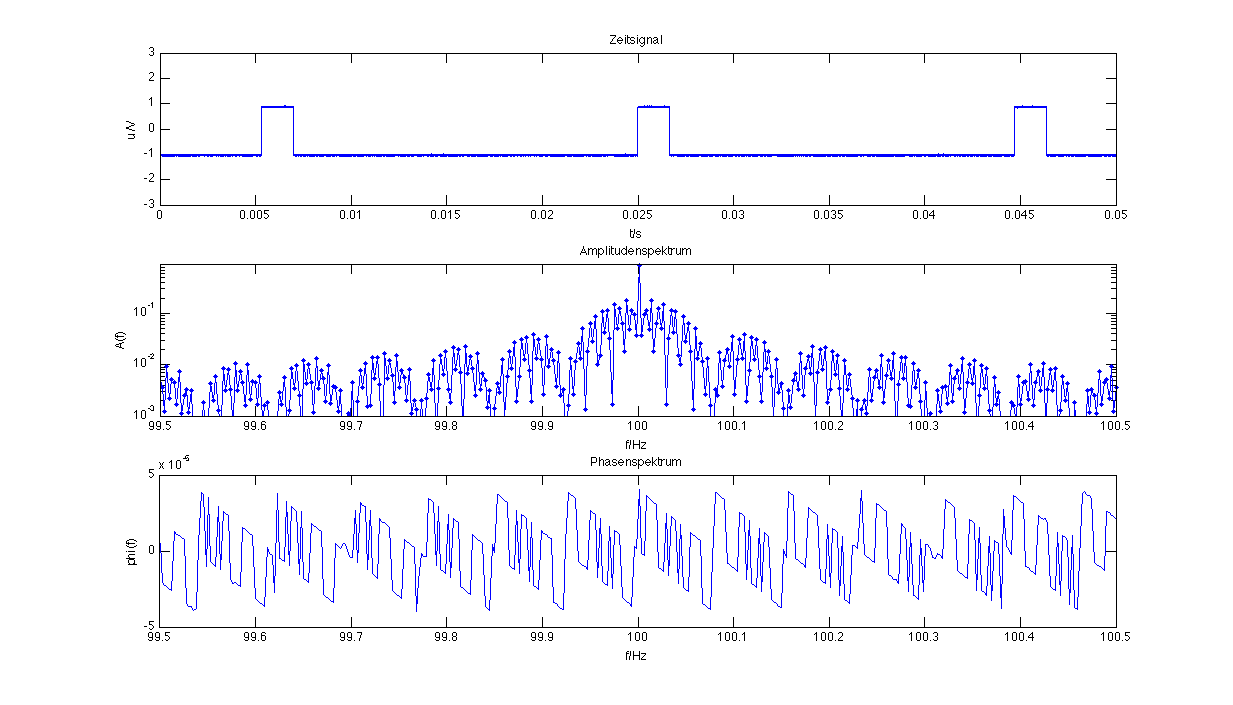
\includegraphics[scale=0.3]{./Bilder/recht_alpha1_-_gemessen.png} %FIXME [width=640px,
                        % height=474px]
                        \caption{Rechtecksignalspektrum für $\aplpha = 0,1$ - gemessen}
                    \end{figure}                
                    
                    \begin{figure}[H]
                        \label{fig:}            
                        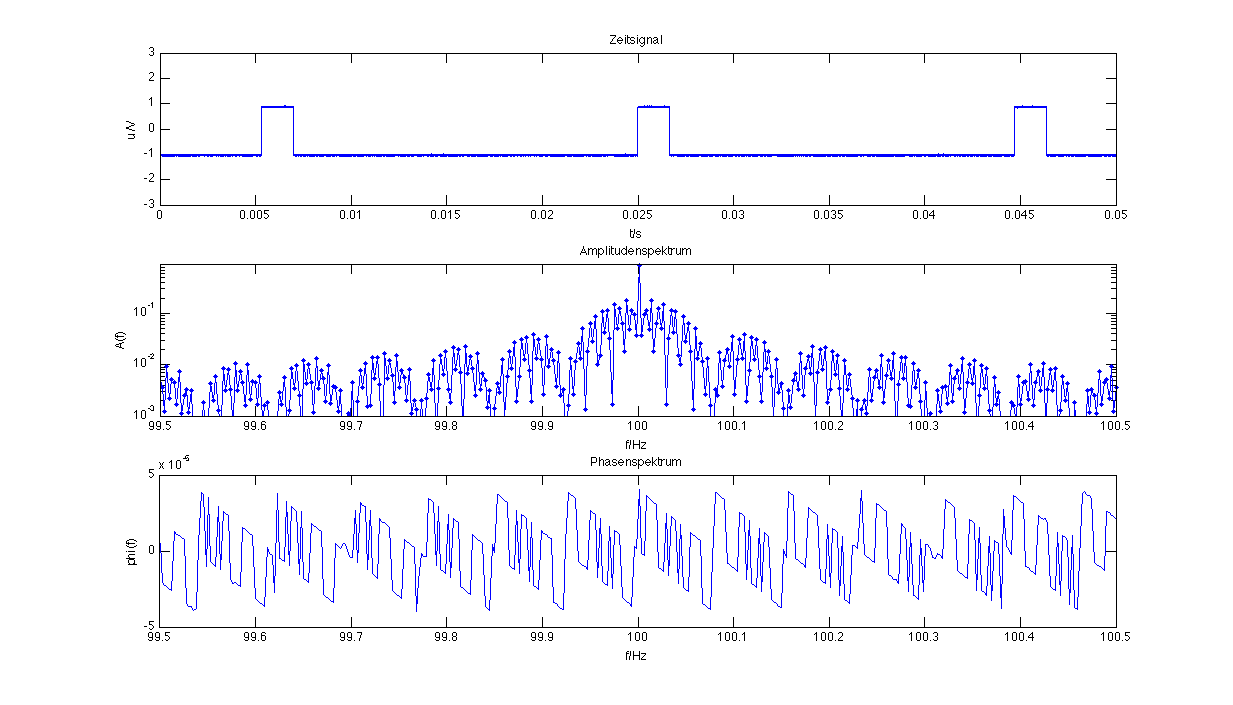
\includegraphics[scale=0.3]{./Bilder/recht_alpha1_-_gemessen.png} %FIXME [width=640px,
                        % height=474px]
                        \caption{Rechtecksignalspektrum für $\aplpha = 0,5$ - gemessen}
                    \end{figure}                

                    \begin{figure}[H]
                        \label{fig:}            
                        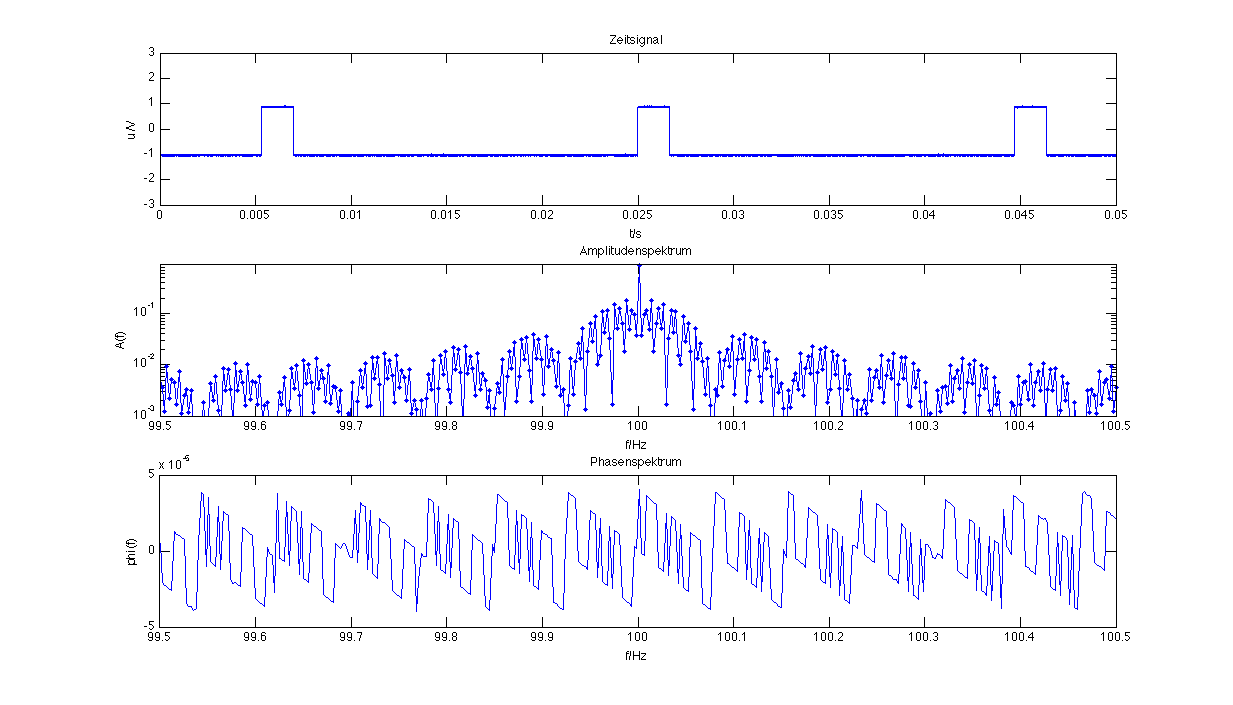
\includegraphics[scale=0.3]{./Bilder/recht_alpha1_-_gemessen.png} %FIXME [width=640px,
                        % height=474px]
                        \caption{Rechtecksignalspektrum für $\aplpha = 0,9$ - gemessen}
                    \end{figure}                
                
                \end{minipage}
                        
            \end{tabular}
            \end{center}
        
    \end{quote}
    
    \subsection{Dreiecksignal}
    \begin{quote}
        
    \end{quote}
    
    \subsection{Cosinussignal}
    \begin{quote}
        
    \end{quote}


    
    


    
        
\end{quote}





%--------------------------------------------------------------------
%--------------------------------------------------------------------            
	
	
	
		
	           \begin{figure}[H]
    			\centering
    				\includegraphics[scale=0.5]{recht_alpha1.png}
    			\caption{Rechecktsignalspektren für $\alpha = 0.1$}
    				\end{figure}		
		\end{center}
		
		Für $\alpha = 0.1$ kann man sehen, dass die Signallängen im Zeitbereich
		deutlich kürzer geworden sind. An der Amplitude ändert sich dabei nichts.
		Dafür ist im Amplitudenspektrum \ldots
		
		\begin{center}
	           \begin{figure}[H]
    			\centering
    				\includegraphics[scale=0.5]{recht_alpha5.png}
    			\caption{Rechecktsignalspektren für $\alpha = 0.5$}		
    			\end{figure}		
    			\end{center}
		
		Für $\alpha = 0.5$ kann man dagegen sehen \ldots
		
		
		\begin{center}
	           \begin{figure}[H]
    			\centering
    				\includegraphics[scale=0.5]{recht_alpha9.png}
    			\caption{Rechecktsignalspektren für $\alpha = 0.9$}		
    			\end{figure}
		\end{center}
		
		Zuletzt sieht man in den Spektren für $\alpha = 0.9$, dass \ldots
		
		\vspace{1em}
		
		

		Die enstandenen Sprektren waren diese:
		
	           \begin{figure}[H]
    			\centering
    				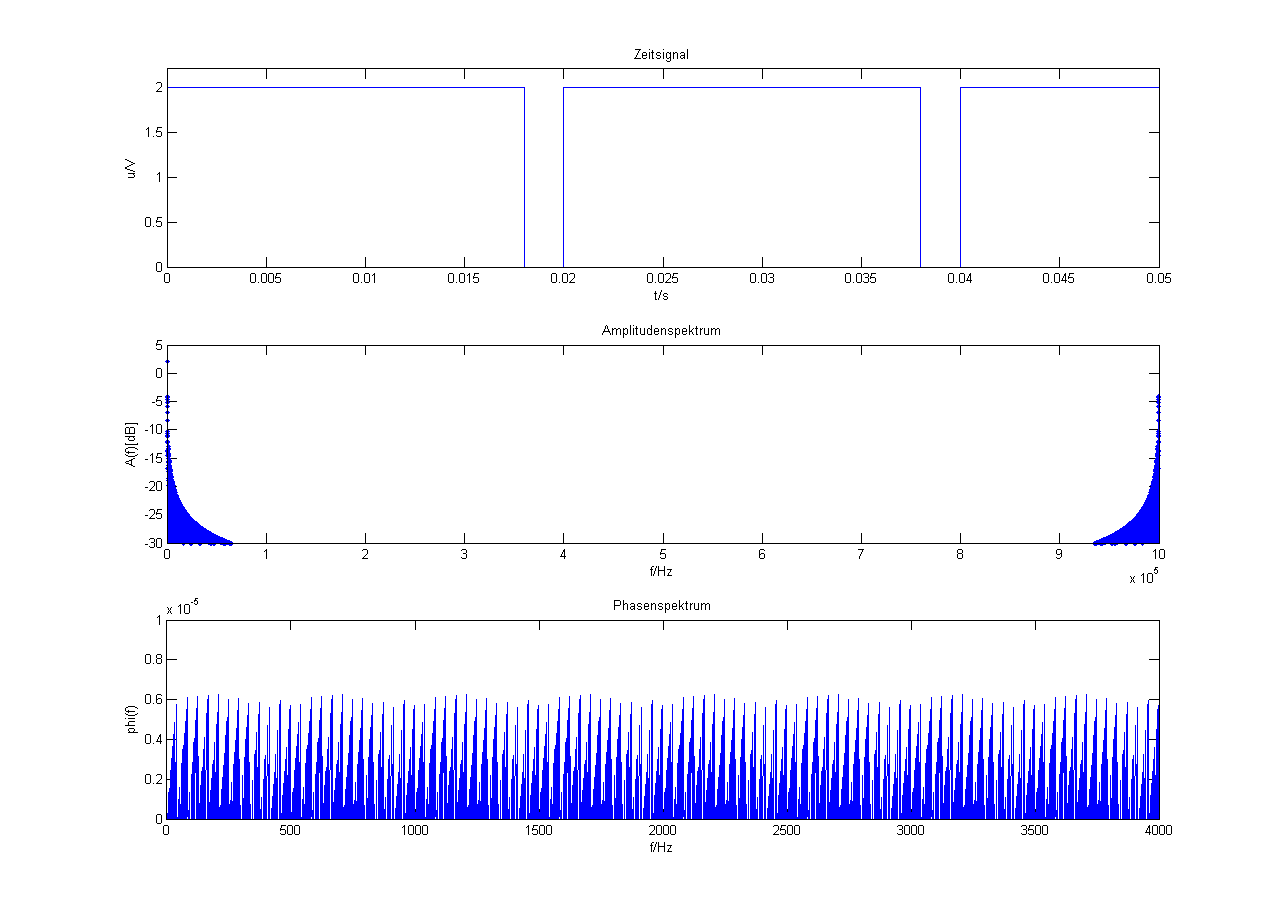
\includegraphics[scale=0.5]{Ampl[dB].png}
    			\caption{Amplitudenspektrum in dB mit limitierter y-Achse}
    			\end{figure}		
		
		
		\vspace{1em}
		
		
		
 Die Ergebnisse folgen:
			
		Dies sind die Spektren mit $\alpha = 0.3$\ldots
			
		\begin{center}
	    
	           \begin{figure}[H]
    			\centering
    				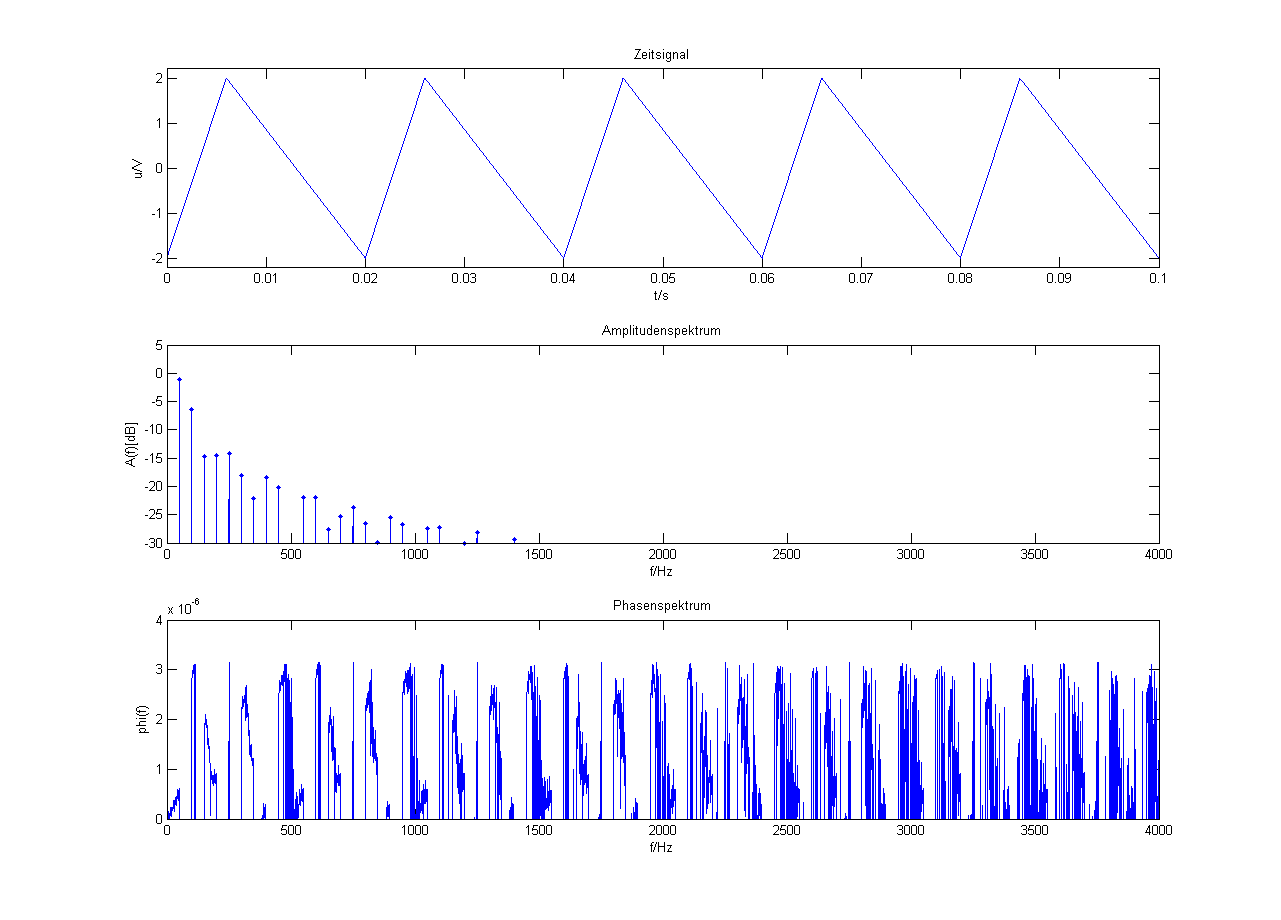
\includegraphics[scale=0.5]{drei_alpha3.png}
    			\caption{Dreiecksignalspektren für $\alpha = 0.3$}
    			\end{figure}		
		
		\end{center}
		
		
		
		\vspace{1em}
		
		Dies sind die Spektren mit $\alpha = 0.5$\ldots
		
		\begin{center}
	    
	           \begin{figure}[H]
    			\centering
    				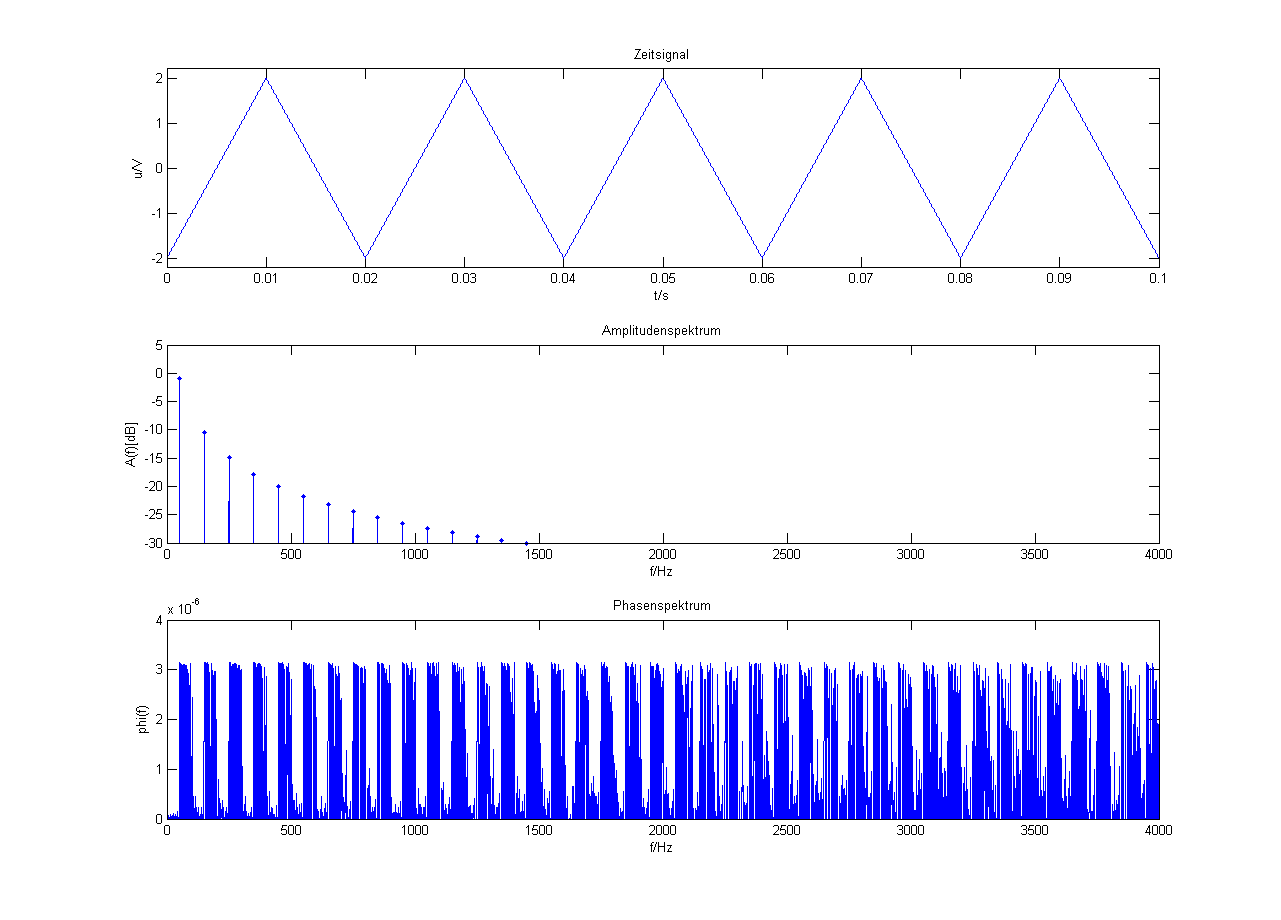
\includegraphics[scale=0.5]{drei_alpha5.png}
    			\caption{Dreiecksignalspektren für $\alpha = 0.5$}
    			\end{figure}		
		
		\end{center}
		
		\vspace{1em}
		
		Und dies sind die Spektren mit $\alpha = 0.9$\ldots
		
		\begin{center}
	    
	           \begin{figure}[H]
    			\centering
    				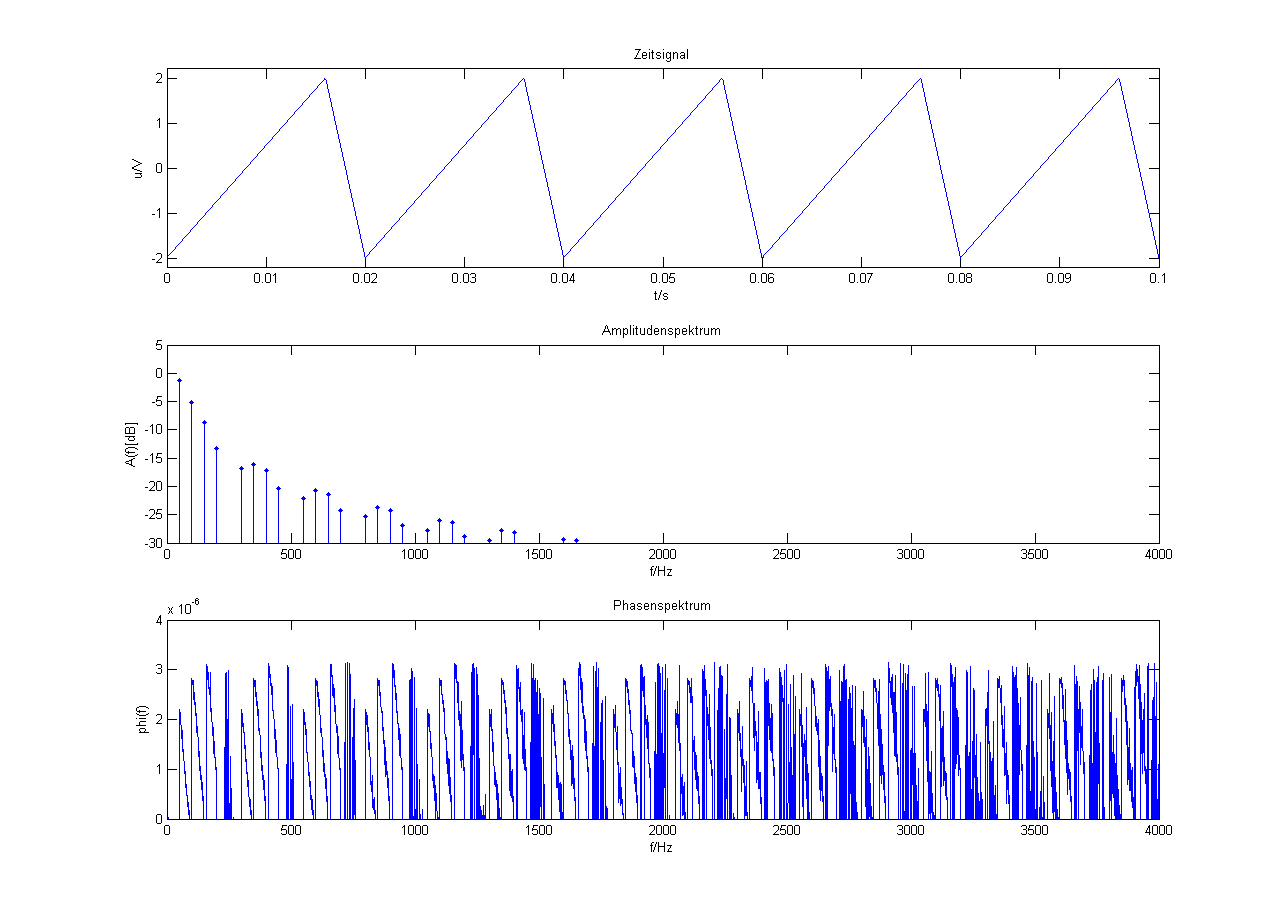
\includegraphics[scale=0.5]{drei_alpha9.png}
    				\caption{Dreiecksignalspektren für $\alpha = 0.9$}
    			\end{figure}		
		
		\end{center}
		
		\vspace{1em}
		
		
		\vspace{1em}
		
 Die
		Ergebnisse ware diese:
		
		Simulation mit $\alpha = 0.1$: \ldots
	
		\begin{center}
	    
	           \begin{figure}[H]
    			\centering
    				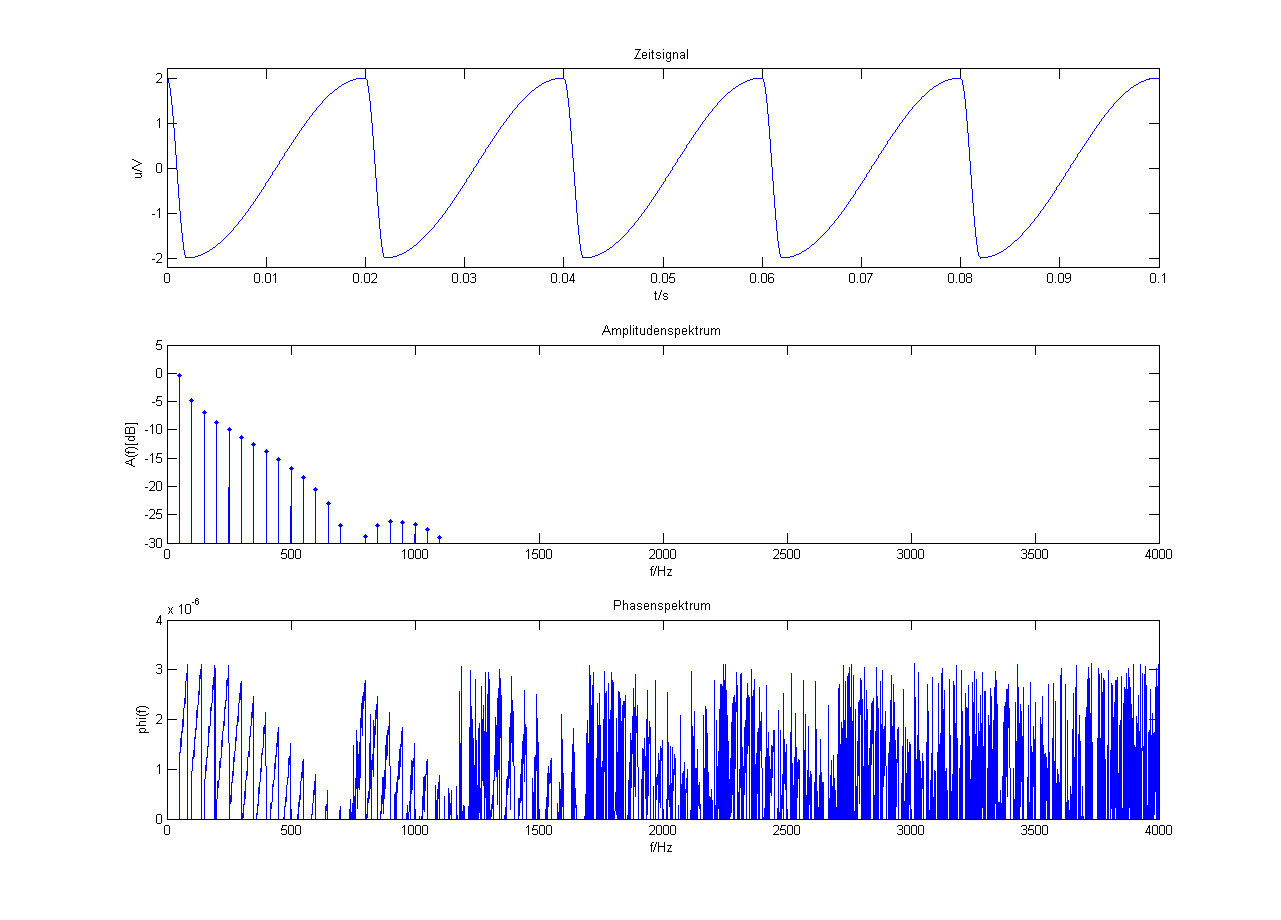
\includegraphics[scale=0.5]{cos_alpha1.png}
    				\caption{Cosinussignalspektren für $\alpha = 0.1$}
    			\end{figure}	
    			\caption{}	
		
		\end{center}
		
		\vspace{1em}
		
		Simulation mit $\alpha = 0.5$: \ldots
		
		\begin{center}
	    
	           \begin{figure}[H]
    			\centering
    				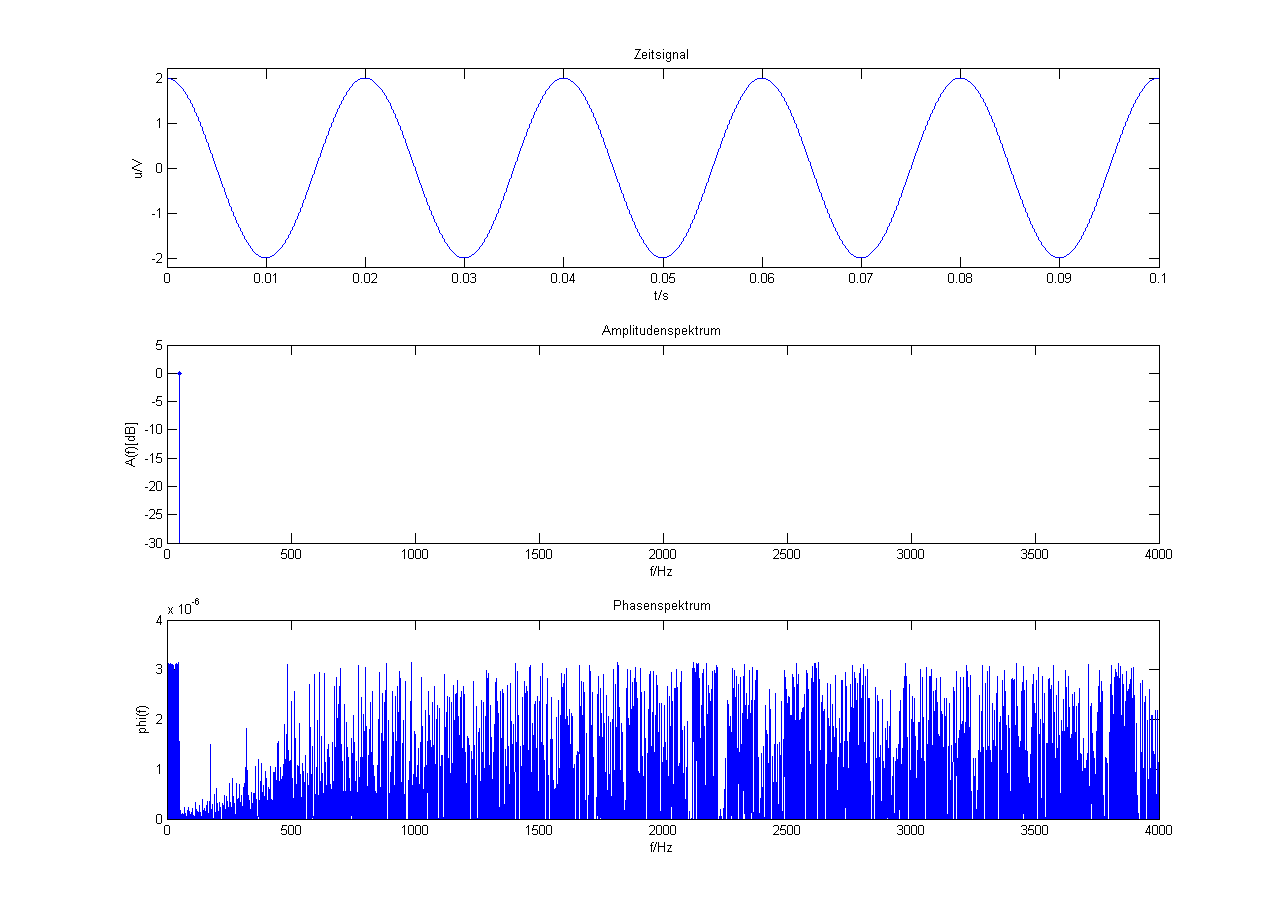
\includegraphics[scale=0.5]{cos_alpha5.png}
    			\caption{Cosinussignalspektren für $\alpha = 0.5$}
    			\end{figure}		
		
		\end{center}
		
		\vspace{1em}
		
		Simulation mit $\alpha = 0.9$: \ldots
		
		\begin{center}
	    
	           \begin{figure}[H]
    			\centering
%    				\includegraphics[scale=0.5]{./Bilder/cos_alpha9.png}
                    \includegraphics[scale=0.5]{cos_alpha9}
    			\caption{Cosinussignalspektren für $\alpha = 0.9$}
    			\end{figure}	
		
		\end{center}
	\begin{quote}	
	\end{quote}
	




%    	\begin{quote}
%            \begin{enumerate}
%      			\item 
%		   \end{enumerate}
%		\end{quote}
%	\end{quote}

%--------------------------------------------------------------------
%--------------------------------------------------------------------
\section{Fazit}
\begin{quote}
     
\end{quote}

%--------------------------------------------------------------------
%--------------------------------------------------------------------
\section{Matlab-Code}
\begin{quote}
    \subsection{Aufgabe1.m bearbeitet}
    \begin{quote}
            \lstinputlisting[
            caption={Aufgabe1 - Matlab-script},
            label=lst:Matlab]
            {./Matlab/Aufgabe1.m}
    \end{quote}
    \subsection{rechteck.m bearbeitet}
    \begin{quote}
            \lstinputlisting[
            caption={Rechteck - Matlab-script},
            label=lst:Matlab]
            {./Matlab/rechteck.m}
    \end{quote}
    \subsection{dreieck.m bearbeitet}
    \begin{quote}
            \lstinputlisting[
            caption={Dreieck - Matlab-script},
            label=lst:Matlab]
            {./Matlab/dreieck.m}        
    \end{quote}
    \subsection{cosinus.m bearbeitet}
    \begin{quote}
            \lstinputlisting[
            caption={Cosinus - Matlab-script},
            label=lst:Matlab]
            {./Matlab/cosinus.m}        
    \end{quote}                 	
\end{quote}


\end{document}